\documentclass[journal]{IEEEtran}

\usepackage{amsmath,amssymb,amsfonts,amsthm}
\usepackage{graphicx}
\usepackage{booktabs}
\usepackage{multirow}
\usepackage{array}
\usepackage{makecell}
\usepackage{microtype}
\usepackage{cite}
\usepackage{url}
\usepackage[hidelinks]{hyperref}

\newcommand{\sys}{AAFV-Net}
\newcommand{\vect}[1]{\mathbf{#1}}
\newtheorem{proposition}{Proposition}
\newtheorem{remark}{Remark}

% =====================================================================================
% AAFV-04 REVISION (prepared in response to the expert review of AAFV-02/AAFV-03).
% Every number in this file is traceable to a logged artifact; see
% AAFV-04_revision/REVIEW_RESPONSE_MATRIX.md and analysis/ for the source of each value.
% Items still required before submission are listed in UNRESOLVED_ISSUES.md.
% =====================================================================================

\begin{document}

\title{AAFV-Net: Reliability-Gated Three-Way Decisions for Adult Cross-Age Face Verification With Audited Random-Impostor False-Accept Risk}

% NOTE FOR SUBMISSION: author order, e-mails, ORCID iDs, corresponding author, and funding
% must be confirmed by all five authors (SUBMISSION_AUTHOR_CHECKLIST.md). Nothing here is fabricated.
\author{Anurag~Nayak,
        Sujal~Chondhekar,
        Sumit~Kumar,
        Piyush~Jain,
        and~Swati~Hira%
\thanks{Manuscript prepared November 2026. This work was carried out at the Indian Institute of Information Technology Nagpur. [Funding statement to be confirmed by the authors.]}%
\thanks{The authors are with the Department of Computer Science and Engineering, Indian Institute of Information Technology Nagpur, Nagpur, Maharashtra, India (e-mail: [to be confirmed]; corresponding author: [to be confirmed]). Code, frozen-artifact hashes, and the test-access log: \url{https://github.com/ImproveMent-Repo/AAFV} [repository URL to be confirmed].}}

\markboth{Submitted to IEEE Transactions on Information Forensics and Security}%
{Nayak \MakeLowercase{\textit{et al.}}: Reliability-Gated Three-Way Decisions for Adult Cross-Age Face Verification}

\maketitle

\begin{abstract}
Cross-age face verification for border control and identity renewal must keep impostor admissions rare while ageing pushes genuine pairs toward the impostor score distribution. We treat it as a three-way decision (auto-accept, manual review, auto-reject) rather than as embedding learning. AAFV-Net fuses five frozen similarity measures computed on the original pair and on age-progressed counterparts from a pre-trained generator. The generated evidence is gated by a synthesis-reliability score and by branch masking during training. A pair is accepted only above a frozen threshold set at the highest guard-passing impostor score on a calibration split. We show that this rule gives a distribution-free, finite-sample false-accept rate (FAR) certificate for exchangeable random impostors without using test data. On person-disjoint MORPH data, the certificate bounds random-impostor FAR at 0.349\% (95\% confidence), and a held-out audit finds 0 false accepts in 1,149 person-disjoint pairs. The system auto-accepts 70.07\% of 24,305 genuine pairs and auto-rejects 98.04\% of 35,735 ArcFace-mined look-alikes, with 5 false accepts. The results are mixed. A guarded ArcFace baseline accepts 89.45\% of genuine pairs with one third of AAFV-Net's manual reviews, and 97.2\% of MORPH genuine pairs span less than five years. On FG-NET adults, AAFV-Net accepts more genuine pairs than ArcFace (51.92\% versus 40.38\%) but falsely rejects 18.20\%. We report the protocol chronology and the experiments still required.
\end{abstract}

\begin{IEEEkeywords}
Biometric verification, cross-age face verification, false-accept rate, reject option, selective classification, conformal risk control, calibration, face age progression.
\end{IEEEkeywords}

% =====================================================================================
\section{Introduction}
\label{sec:intro}
\IEEEPARstart{F}{ace} verification across long time spans is required when a traveller is compared with an older passport photograph, when a national credential is renewed, or when a forensic examiner compares a probe with archived images~\cite{grother2019frvt_part3,bestrowden2018longitudinal}. Ageing changes facial texture, soft tissue, and, in children, skeletal shape~\cite{lanitis2002fgnet,deb2018child}. For a fixed matcher, genuine similarity therefore decreases as the elapsed time grows~\cite{bestrowden2018longitudinal}, while the impostor score distribution does not. A single decision threshold must then trade false accepts against false rejects, and in high-assurance settings the two errors have very different costs: an admitted impostor is a security failure, whereas a rejected genuine user can be resolved by a human examiner~\cite{phillips2018pnas}.

Most research on age-invariant face recognition (AIFR) addresses the representation. Discriminative methods remove age information from identity features~\cite{wang2018oecnn,wang2019dal,huang2021mtlface}; AIM learns cross-age synthesis and recognition jointly~\cite{zhao2022aim}; OrdCon learns age features that follow the ordinal direction of ageing and improves cross-dataset accuracy~\cite{wang2025ordcon}. These works report identification accuracy or verification accuracy at a threshold chosen on the evaluation protocol. They do not address how a deployed system should choose its operating points from finite data, what false-accept guarantee those operating points carry, or which pairs it should defer to a human.

The decision side has its own literature. Chow's reject option~\cite{chow1970reject,herbei2006reject} and selective classification~\cite{elyaniv2010selective,geifman2017selective} trade coverage for risk; conformal prediction and conformal risk control give distribution-free finite-sample guarantees under exchangeability~\cite{vovk2005alrw,angelopoulos2024crc,angelopoulos2021ltt}; and biometric evaluation practice prescribes how to estimate error rates when comparisons share subjects~\cite{bolle2004subsets,schuckers2010book,iso19795_1}. Biometric score fusion is mature~\cite{kittler1998combining,ross2003fusion,nandakumar2008lr}, including quality-dependent fusion with missing channels~\cite{poh2009quality}. What is missing, to our knowledge, is a cross-age verification study that (i) states the operational objective as a three-way decision with an explicit false-accept guarantee, (ii) uses generated age-progression evidence only as an auxiliary, reliability-gated channel, and (iii) evaluates the result under a logged test budget and an external dataset, reporting where the guarantee and the design fail.

\textbf{Research question.} \emph{Can a lightweight fusion of frozen similarity measures and reliability-gated age-progression evidence support a three-way cross-age verification policy whose random-impostor false-accept rate is certified from calibration data and confirmed on held-out data, while automating a useful share of genuine and look-alike decisions?}

\textbf{Contributions.} We separate what is supported from what is not.
\begin{enumerate}
\item \emph{A three-way cross-age verification policy with a calibration-side FAR certificate.} We formalize the accept rule (highest guard-passing calibration impostor score plus a margin) and show, by a standard order-statistic argument, that it bounds the random-impostor FAR at $0.349\%$ with 95\% confidence from 1,170 person-disjoint calibration impostors, without using the test set (Proposition~\ref{prop:cert}). A held-out audit (0/1,149) agrees. We quantify the sample sizes needed for operational targets (Table~\ref{tab:samplesize}).
\item \emph{An empirical account of why guards matter.} Under the same zero-false-accept rule, every variant without branch-probability guards, and three learned end-to-end comparators, place the accept threshold at or above $0.98$ and accept at most $0.27\%$ of genuine calibration pairs, whereas the guarded system accepts $74.13\%$ of the same pairs (Tables~\ref{tab:cal_subset}, \ref{tab:ablations}).
\item \emph{Reliability-gated age-progression evidence.} Age-progressed comparisons enter only through a separate branch weighted by a synthesis-reliability score and trained with branch masking. Ablations show that masking is necessary in this design; the added value of the shared-target grid over endpoint progression is not established (Section~\ref{sec:ablation}).
\item \emph{A transparent evaluation, including negative results.} We reconcile all evaluation populations (Table~\ref{tab:populations}), reconstruct the protocol chronology (Table~\ref{tab:chronology}), report calibration diagnostics, operational workload, the MORPH age-gap deficit relative to ArcFace, and the failure of the false-reject budget on FG-NET.
\end{enumerate}
We do not claim a new face representation, superiority over ArcFace on MORPH genuine acceptance, robustness to morphing or presentation attacks, or validity for children.

The paper is organized as follows. Section~\ref{sec:related} reviews related work and positions each component. Section~\ref{sec:formulation} defines the problem and threat model. Section~\ref{sec:risk} derives the risk statements. Section~\ref{sec:method} specifies \sys. Section~\ref{sec:protocol} describes data, splits, and the protocol chronology. Section~\ref{sec:results} reports results, and Sections~\ref{sec:discussion}--\ref{sec:conclusion} discuss limitations and conclude.

% =====================================================================================
\section{Related Work}
\label{sec:related}

\subsection{Age-Invariant Face Recognition}
Early AIFR used discriminative subspaces~\cite{li2011aifr}. Deep methods decompose features into identity and age components (OE-CNN~\cite{wang2018oecnn}), decorrelate them adversarially (DAL~\cite{wang2019dal}), or add an ageing task (MTLFace~\cite{huang2021mtlface}). AIM~\cite{zhao2022aim} couples an attention-based synthesis network with disentangled representation learning, evaluates identity preservation with a user study and recognition benchmarks (MORPH, CACD-VS, FG-NET, IJB-C), and introduces the CAFR benchmark. OrdCon~\cite{wang2025ordcon} contrasts direction vectors between features of younger and older faces with the ageing direction and adds a soft proxy-matching loss; it reports homogeneous and cross-dataset results on MORPH, FG-NET, and AgeDB and openly notes where dataset-specific methods outperform it. These methods change the representation; \sys\ keeps the representations frozen and changes the decision. The two are complementary: an AIFR embedding could replace ArcFace inside \sys, which we have not tested. Large-margin matchers such as CosFace~\cite{wang2018cosface}, ArcFace~\cite{deng2019arcface}, MagFace~\cite{meng2021magface}, and AdaFace~\cite{kim2022adaface} remain the strongest generic baselines; only ArcFace is evaluated here.

\subsection{Face Age Progression and Identity Preservation}
Conditional generators progressed from CAAE~\cite{zhang2017caae} and IPCGANs~\cite{tang2018ipcgan} to PFA-GAN~\cite{huang2021pfagan} and SAM~\cite{alaluf2021sam}, which regresses StyleGAN2~\cite{karras2020stylegan2} latent codes towards a target age. Generators can alter identity, particularly for large changes or young children~\cite{deb2018child}. AIM measures this with a user study~\cite{zhao2022aim}. We use SAM unchanged and treat its outputs as noisy evidence; we have not yet measured identity preservation with a recognizer outside the pipeline (Section~\ref{sec:limitations}).

\subsection{Score Fusion, Quality, and Uncertainty}
Classical fusion combines matcher scores by fixed rules, density ratios, or learned classifiers~\cite{kittler1998combining,ross2003fusion,nandakumar2008lr}. Poh \emph{et al.}~\cite{poh2009quality} benchmarked quality-dependent and cost-sensitive fusion with missing modalities, which is the closest precedent for our reliability-weighted auxiliary branch. Probabilistic and quality-aware embeddings model per-sample uncertainty~\cite{shi2019pfe,meng2021magface,kim2022adaface,ahn2024ucface}. Our fusion is a small learned combiner of this family; its distinguishing element is that one input channel is synthetic and is gated by an explicit reliability score.

\subsection{Calibration}
Platt scaling~\cite{platt1999}, isotonic regression~\cite{zadrozny2002isotonic}, and temperature scaling~\cite{guo2017calibration} map scores to probabilities; ECE~\cite{naeini2015ece}, Brier score~\cite{brier1950}, and negative log-likelihood measure the result. Xu \emph{et al.}~\cite{xu2024asc} calibrate face and kinship verification scores. All of these are monotone maps; a threshold on a calibrated score is a threshold on the raw score. This observation determines what calibration can and cannot contribute to our decision rule (Section~\ref{sec:calib_role}).

\subsection{Reject Option, Selective Classification, and Risk Control}
Chow derived the optimal error--reject trade-off for known posteriors~\cite{chow1970reject}; later work studies learning with rejection~\cite{herbei2006reject} and selective deep classifiers with risk--coverage guarantees~\cite{elyaniv2010selective,geifman2017selective}. Split-conformal methods and their risk-control extensions provide finite-sample guarantees under exchangeability~\cite{vovk2005alrw,angelopoulos2024crc,angelopoulos2021ltt}, with weighted variants for covariate shift~\cite{tibshirani2019covshift}. Our accept rule is a special case of this machinery (a maximum order statistic), and our reject rule is a conformal-style quantile; we use these results rather than claim them.

\subsection{Error-Rate Estimation, Hard Impostors, Fairness, and Attacks}
Zero-failure bounds follow from the binomial model~\cite{clopper1934,hanley1983rule3}; comparisons that share subjects require subset or cluster resampling~\cite{bolle2004subsets,schuckers2010book}. Look-alikes and twins raise false-match rates substantially~\cite{paone2014twins}. Accuracy varies with sex, age, and race~\cite{klare2012demographics,grother2019frvt_part3,krishnapriya2020race}. Morphing and presentation attacks~\cite{scherhag2019morph,iso30107_3} require dedicated detectors and are outside our threat model. Table~\ref{tab:positioning} summarizes, component by component, what \sys\ adopts, modifies, or adds.

\begin{table*}[t]
\centering
\caption{Component-Level Positioning. ``Adopted'' Components Are Used Unchanged; ``Modified'' Components Are Adapted; ``New'' Marks Elements We Could Not Find in the Cited Literature in This Combination. The Evidence Column States What Currently Supports Each Element.}
\label{tab:positioning}
\footnotesize
\setlength{\tabcolsep}{3pt}
\begin{tabular}{@{}p{3.1cm}p{4.0cm}p{1.3cm}p{8.4cm}@{}}
\toprule
\textbf{Component} & \textbf{Closest prior work} & \textbf{Status} & \textbf{Evidence in this paper and remaining gap} \\
\midrule
Identity / similarity extractors & ArcFace~\cite{deng2019arcface}, VGG-Face~\cite{parkhi2015vgg}, EfficientNet~\cite{tan2019efficientnet}, LPIPS~\cite{zhang2018lpips}, SSIM~\cite{wang2004ssim} & Adopted & Frozen, pre-trained. EfficientNet is redundant (dropping it raises calibration accept, Table~\ref{tab:ablations}). \\
Age progression & SAM~\cite{alaluf2021sam}; joint synthesis--recognition in AIM~\cite{zhao2022aim} & Adopted & Frozen generator; identity preservation not independently measured (Section~\ref{sec:limitations}). \\
Shared-target 5-year grid & Endpoint progression~\cite{zhao2022aim,huang2021pfagan} & New (design) & Reduces test accept $83.91\%\to70.07\%$; neutral hard rejection $53.98\%\to57.49\%$ with overlapping 95\% CIs. Benefit not established. \\
Reliability score $R_{\text{sam}}$ and branch masking & Quality-dependent fusion with missing channels~\cite{poh2009quality} & Modified & Masking is necessary in this recipe (accept $3.60\%$ without it); removing $R_{\text{sam}}$ changes calibration accept by $<1$~pp. Missing-branch inference test not run. \\
Fusion MLP + Platt & Score fusion~\cite{kittler1998combining,ross2003fusion,nandakumar2008lr}; Platt~\cite{platt1999} & Adopted & Platt is monotone, so decisions are invariant to it except through the branch floors $\rho$ (Section~\ref{sec:calib_role}). \\
Accept rule: zero-FA order statistic with guards & Selective classification~\cite{geifman2017selective,elyaniv2010selective}; conformal risk control~\cite{vovk2005alrw,angelopoulos2024crc} & Modified & Guards are the mechanism that avoids $T_{\text{acc}}>1$ (all guard ablations give 0\% accept). The finite-sample certificate (Proposition~\ref{prop:cert}) follows from known order-statistic arguments. \\
Reject rule $T_{\text{rej}}(\beta)$ & Chow~\cite{chow1970reject}; conformal quantiles~\cite{vovk2005alrw} & Adopted & Holds on MORPH test ($0.54\%\le1\%$) but fails under shift: $18.20\%$ false rejects on FG-NET adults. \\
Audit protocol (quarantine, hashes, look budget) & ISO/IEC 19795-1~\cite{iso19795_1}; subset bootstrap~\cite{bolle2004subsets} & Modified & Logged; adaptivity between looks not excluded (Table~\ref{tab:chronology}). \\
\bottomrule
\end{tabular}
\end{table*}


% =====================================================================================
\section{Problem Formulation and Threat Model}
\label{sec:formulation}

\subsection{Notation and Decision Rule}
A comparison is a pair of aligned face images $(I_1,I_2)$ with ages $a_1\le a_2$, age gap $\Delta a=a_2-a_1$, and label $y=1$ for the same person and $y=0$ otherwise. A scorer maps the pair to a feature vector $\vect{z}$ (Table~\ref{tab:features}) and to a fused probability $P\in(0,1)$; two branch probabilities $P_d,P_s$ and a guard indicator $\mathcal{G}(\vect{z})\in\{0,1\}$ are also computed (Section~\ref{sec:method}). With two frozen thresholds $T_{\text{rej}}<T_{\text{acc}}$, the decision is
\begin{equation}
\label{eq:decision_rule}
\delta(\vect{z})=
\begin{cases}
\text{Accept}, & \mathcal{G}(\vect{z})=1 \text{ and } P\ge T_{\text{acc}},\\
\text{Reject}, & P< T_{\text{rej}},\\
\text{Review}, & \text{otherwise.}
\end{cases}
\end{equation}
Guards can only move a candidate accept to review; they never cause acceptance or rejection.

\subsection{Operational Objectives}
For a population of comparisons, define the false-accept rate $\text{FAR}=\Pr(\delta=\text{Accept}\mid y=0)$, the genuine false-reject rate $\text{FRR}_X=\Pr(\delta=\text{Reject}\mid y=1)$, the genuine coverage $C=\Pr(\delta=\text{Accept}\mid y=1)$, and the review rate. The design objective is
\begin{equation}
\label{eq:objective}
\max\; C \quad \text{s.t.}\quad \text{FAR}\le\varepsilon,\;\; \text{FRR}_X\le\beta ,
\end{equation}
where $\varepsilon$ must be certified with confidence $1-\delta$ and $\beta$ is a target. The review rate is the price paid for both constraints, so we report it explicitly (Section~\ref{sec:workload}).

\subsection{Threat Model and Population}
Table~\ref{tab:threat} lists the adversaries considered. The certified statement covers zero-effort random impostors of the same sex drawn from the same population as the calibration data. Look-alike impostors are evaluated empirically only, because mined pairs are by construction not a random sample. Morphing, digital manipulation, and presentation attacks are out of scope. The operational population is adults ($a\ge16$); this restriction was introduced after observing pediatric false accepts on FG-NET (Section~\ref{sec:fgnet}).

\begin{table}[t]
\centering
\caption{Threat Model and Evidential Status of Each Claim.}
\label{tab:threat}
\footnotesize
\setlength{\tabcolsep}{2.5pt}
\resizebox{\columnwidth}{!}{%
\begin{tabular}{@{}p{0.34\columnwidth}p{0.24\columnwidth}p{0.42\columnwidth}@{}}
\toprule
\textbf{Adversary / condition} & \textbf{Status} & \textbf{Evidence} \\
\midrule
Zero-effort random impostor, same sex, adult, MORPH-like capture & In scope; certified & Prop.~\ref{prop:cert} (calibration) and 0/1,149 test audit \\
Look-alike impostor mined by ArcFace & In scope; empirical only & $5/35{,}735$ FA; mining matches training negatives (Sec.~\ref{sec:hard}) \\
Look-alike mined by other models & In scope; empirical only & Neutral set, 57.49\% auto-rejected, 0 FA \\
Low-quality or degraded probe & Partly in scope & Quality guard exists; no degradation stress test \\
Unconstrained capture (pose, scan, era) & Partly in scope & FG-NET adults only (82 persons) \\
Children ($a<16$) & Out of scope & 4/20,000 FA on FG-NET, all involving ages 0--4 \\
Morphing, digital manipulation, presentation attacks~\cite{scherhag2019morph,iso30107_3} & Out of scope & Not evaluated; requires separate PAD/MAD \\
\bottomrule
\end{tabular}}
\end{table}


% =====================================================================================
\section{Risk Statements and Their Assumptions}
\label{sec:risk}

\subsection{Accept Side: A Calibration Certificate}
Let $s(\vect{z})=P$ if $\mathcal{G}(\vect{z})=1$ and $s(\vect{z})=-\infty$ otherwise, so that $\delta=\text{Accept}$ exactly when $s\ge T_{\text{acc}}$. On the calibration split, $T_{\text{acc}}$ is set above the largest $s$ over all impostor calibration pairs, which include the person-disjoint random pool $\mathcal{D}^{\text{cal}}_{\text{random}}$ of size $n$.

\begin{proposition}
\label{prop:cert}
Assume that the scorer, the guards, and the threshold rule are fixed independently of $\mathcal{D}^{\text{cal}}_{\text{random}}$, and that the $n$ scores $s_1,\dots,s_n$ of $\mathcal{D}^{\text{cal}}_{\text{random}}$ and the score $s_{\text{new}}$ of a future random impostor pair are independent and identically distributed. Then for any threshold $T\ge\max_i s_i$,
\begin{align}
\label{eq:cert_exp}
\mathbb{E}\big[\text{FAR}(T)\big] &\le \frac{1}{n+1},\\
\label{eq:cert_pac}
\Pr\big[\text{FAR}(T)>\varepsilon\big] &\le (1-\varepsilon)^{n}.
\end{align}
\end{proposition}
\begin{proof}[Sketch]
$\text{FAR}(T)\le F(\max_i s_i)$, where $F(t)=\Pr(s_{\text{new}}\ge t)$. For (\ref{eq:cert_exp}), $s_{\text{new}}$ exceeds all $n$ exchangeable values with probability at most $1/(n+1)$~\cite{vovk2005alrw}. For (\ref{eq:cert_pac}), $F(\max_i s_i)>\varepsilon$ requires all $n$ scores to fall below the upper-$\varepsilon$ quantile of the score distribution, which has probability at most $(1-\varepsilon)^n$.
\end{proof}

Setting the right side of (\ref{eq:cert_pac}) to $\delta$ gives $\varepsilon=1-\delta^{1/n}$. With $n=1{,}170$ and $\delta=0.05$, $\varepsilon=0.256\%$. The floor $\rho$ was selected from three values on the calibration split; a union bound over the three settings replaces $\delta$ by $\delta/3$ and gives $\varepsilon=0.349\%$, which we report as the calibration certificate. The expected-FAR bound (\ref{eq:cert_exp}) is $0.085\%$. Because $T_{\text{acc}}$ is also above the impostor maximum of the larger correlated pools, the true FAR is likely smaller. Those pools cannot strengthen the certificate without a model of their dependence.

\begin{remark}
The certificate needs the calibration data but not the test data. It therefore holds for the Look-1 and Look-2 checkpoints separately, whatever happened between the two test looks. It does not cover look-alikes, other capture conditions, or other demographic mixes: these violate the identical-distribution assumption.
\end{remark}

\subsection{Accept Side: Held-Out Audit}
On a separate set of $N$ person-disjoint test impostors with $k=0$ observed false accepts, the exact one-sided Clopper--Pearson bound is $1-\alpha^{1/N}$~\cite{clopper1934,hanley1983rule3}. With $N=1{,}149$: $0.260\%$ at $\alpha=0.05$, and $0.320\%$ when $\alpha$ is split over the two looks. The audit is an independent check of the certificate on new persons; it is not the source of the guarantee.

\subsection{Independence, Dependence, and Sample Size}
\label{sec:dependence}
In $\mathcal{D}_{\text{random}}$ each person contributes one image to exactly one pair (\texttt{pairs.d\_random}: 2,298 distinct persons for 1,149 pairs; 982 male and 167 female pairs). Conditional on the frozen model, trials share no subject. Residual dependence can remain through shared acquisition conditions in MORPH (one booking environment). If such dependence reduces the effective number of trials by a design effect $D$, the $\alpha=0.025$ audit bound becomes $1-0.025^{D/1149}$: $0.48\%$ for $D=1.5$ and $0.64\%$ for $D=2$. $\mathcal{D}_{\text{all\_random}}$ (pairs drawn with replacement, repeated persons), $\mathcal{D}_{\text{hard}}$, the neutral set, and FG-NET (at most 82 persons) are reported as empirical counts with person-clustered bootstrap intervals, never as binomial bounds. Table~\ref{tab:samplesize} gives the number of independent comparisons required for operational targets: certifying $10^{-4}$ with zero errors requires about 30,000 independent pairs (about 60,000 persons in our design), roughly 26 times the current test pool. The present certificate therefore supports a statement at the $10^{-3}$ scale, not at the $10^{-4}$ to $10^{-5}$ levels typical of border-control requirements.

\begin{table}[t]
\centering
\caption{Independent Impostor Comparisons $N$ Required to Certify $\text{FAR}\le\varepsilon$ With $k$ Observed False Accepts (Exact One-Sided Clopper--Pearson, $\alpha=0.05$), and the Persons Needed Under the Person-Disjoint Design of $\mathcal{D}_{\text{random}}$.}
\label{tab:samplesize}
\footnotesize
\setlength{\tabcolsep}{3.5pt}
\begin{tabular}{@{}lcccc@{}}
\toprule
\textbf{Target $\varepsilon$} & $k=0$ & $k=1$ & $k=2$ & \textbf{Persons ($k=0$)} \\
\midrule
$10^{-3}$ & 2,995 & 4,742 & 6,294 & 5,990 \\
$10^{-4}$ & 29,956 & 47,437 & 62,956 & 59,912 \\
$10^{-5}$ & 299,572 & 474,385 & 629,578 & 599,144 \\
\midrule
\multicolumn{5}{@{}p{0.95\columnwidth}@{}}{\footnotesize This work: $N=1{,}149$, $k=0$ gives $\varepsilon=0.260\%$ ($\alpha=0.05$) or $0.320\%$ ($\alpha/2$).}
\end{tabular}
\end{table}


\subsection{Reject Side}
$T_{\text{rej}}(\beta)$ is the empirical $\beta$-quantile of fused probabilities over genuine calibration pairs. If genuine pairs were exchangeable, the expected false-reject rate would be at most $\lceil\beta(n_g+1)\rceil/(n_g+1)$~\cite{vovk2005alrw}. Genuine calibration pairs are not exchangeable, because one person contributes many pairs, so this is an approximation within MORPH. Section~\ref{sec:fgnet} shows that it fails under dataset shift.

% =====================================================================================
\section{Method}
\label{sec:method}

\begin{figure*}[t]
\centering
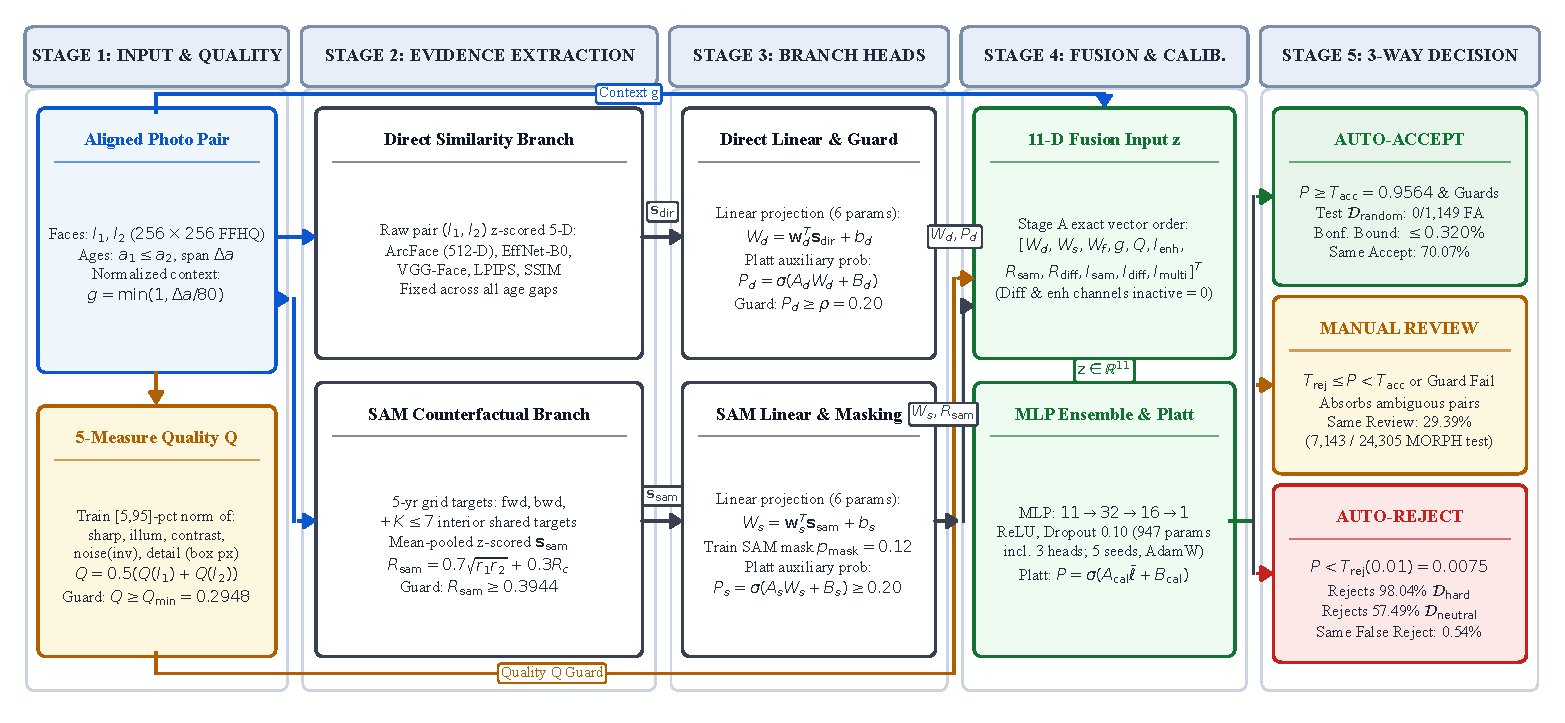
\includegraphics[width=\textwidth]{figures/fig2_architecture.pdf}
\caption{\sys\ as evaluated (Stage~A). (1) Alignment to $256\times256$ FFHQ geometry and five-measure quality $Q$. (2) Five similarity measures on the original pair (direct branch) and on SAM age-progressed pairs at grid targets, with reliability $R_{\text{sam}}$. (3) One linear head per branch with Platt-scaled branch probabilities; SAM masking during training. (4) The 11-D vector of Table~\ref{tab:features} feeds a 5-seed MLP ensemble and Platt calibration. (5) The guarded three-way rule (\ref{eq:decision_rule}). Rates shown are MORPH test Look~2.}
\label{fig:architecture}
\end{figure*}

\subsection{Alignment and Image Quality}
Faces are detected (dlib HOG with an SCRFD fallback), aligned to $256\times256$ FFHQ geometry, and scored by five measures (\texttt{quality.py}): Laplacian variance, luminance balance $1-|\bar{g}-128|/128$, grey-level standard deviation, the Immerk{\ae}r noise estimate (inverted), and detected face-box size. Each measure is clipped to its 5th--95th percentile range on \texttt{train\_fit} and scaled to $[0,1]$, giving $\tilde q_m(I)$, and
\begin{equation}
\label{eq:quality}
Q(I)=\frac{1}{5}\sum_{m=1}^{5}\tilde q_m(I),\qquad Q=\tfrac12\big(Q(I_1)+Q(I_2)\big).
\end{equation}

\subsection{Similarity Measures and Branches}
For an image pair $(A,B)$ the five-score vector is $\vect{s}(A,B)=[s_{\text{arc}},s_{\text{eff}},s_{\text{vgg}},d_{\text{lpips}},s_{\text{ssim}}]^{\top}$: cosine similarities of ArcFace (InsightFace \texttt{buffalo\_l})~\cite{deng2019arcface}, EfficientNet-B0~\cite{tan2019efficientnet}, and VGG-Face~\cite{parkhi2015vgg} descriptors, the LPIPS (AlexNet) distance~\cite{zhang2018lpips}, and grey-level SSIM~\cite{wang2004ssim}. Scores are z-standardized with \texttt{train\_fit} statistics.

\emph{Direct branch:} $\vect{s}_{\text{dir}}$ is the standardized $\vect{s}(I_1,I_2)$.
\emph{SAM branch:} target ages are snapped to a 5-year grid; the younger image is progressed to $t_{\text{fwd}}=\text{snap}(a_2)$, the older one regressed to $t_{\text{bwd}}=\text{snap}(a_1)$, and both are rendered at up to $K_{\max}=7$ interior grid ages $t_k\in(a_1,a_2)$. With standardized comparison vectors $\vect{z}_{\text{fwd}},\vect{z}_{\text{bwd}},\vect{z}_{\text{sh},k}$ and $\vect{b}=\frac12(\vect{z}_{\text{fwd}}+\vect{z}_{\text{bwd}})$,
\begin{equation}
\vect{s}_{\text{sam}}=
\begin{cases}
\tfrac12\vect{b}+\tfrac12\,\tfrac{1}{K_{\text{used}}}\sum_{k}\vect{z}_{\text{sh},k}, & K_{\text{used}}\ge1,\\
\vect{b}, & K_{\text{used}}=0,
\end{cases}
\end{equation}
and $\vect{s}_{\text{sam}}=\vect{0}$ when either endpoint synthesis is unavailable ($I_{\text{sam}}=0$). Missing generations are masked, never imputed (\texttt{pairvec.py}).

\subsection{Synthesis Reliability}
Each generated face receives $r_t=\frac13 R_i+\frac13 R_a+\frac13 Q(\hat I)$, where $R_i=\max(0,\cos(f_{\text{arc}}(\hat I),f_{\text{arc}}(I)))$ measures identity agreement with its source, $R_a=1-\min\!\big(1,\max(0,|\hat a-b_{\text{pair}}-t|-\epsilon)/(2\epsilon)\big)$ measures age accuracy with an age estimator after removing the pair's estimation bias $b_{\text{pair}}$, and $Q(\hat I)$ is image quality. Averaging $r_t$ over each face's syntheses gives $r_1,r_2$; with $\sigma_{\text{arc}}$ the spread of ArcFace cosines across targets and $\sigma_{\max}$ its \texttt{train\_fit} 95th percentile,
\begin{equation}
\label{eq:rsam}
R_{\text{sam}}=0.7\sqrt{r_1r_2}+0.3\big(1-\min(1,\sigma_{\text{arc}}/\sigma_{\max})\big),
\end{equation}
and $R_{\text{sam}}=0$ when SAM is unavailable. $R_i$ uses ArcFace, which is also a fusion input; this circularity is discussed in Section~\ref{sec:limitations}.

\subsection{Fusion, Branch Masking, and Training}
Linear heads produce $W_d=\vect{w}_d^{\top}\vect{s}_{\text{dir}}+b_d$ and $W_s=\vect{w}_s^{\top}\vect{s}_{\text{sam}}+b_s$, and separate Platt scalers fitted on \texttt{train\_val} give $P_d=\sigma(A_dW_d+B_d)$ and $P_s=\sigma(A_sW_s+B_s)$. The fusion input $\vect{z}$ is defined completely in Table~\ref{tab:features}. Four of its eleven entries are constant in the evaluated system; they are placeholders for an enhancement and a diffusion branch that were not built, they do not affect any output, and an output-identical 7-input network exists. An MLP $11\to32\to16\to1$ with ReLU and dropout $0.1$ has 929 weights; with the three 6-parameter heads, 947 per seed. Five seeds are trained on \texttt{train\_fit} with AdamW (learning rate $3\times10^{-3}$ and weight decay $10^{-2}$, chosen from a $2\times2$ grid by \texttt{train\_val} log-loss), batch size 2,048, up to 100 epochs, and early stopping on \texttt{train\_val} log-loss (patience 10). Pairs are weighted by inverse age-gap-bin frequency.

\emph{Training negatives.} For each split, impostor training pairs number three times the genuine pairs, half drawn at random and half from the five most ArcFace-similar same-sex images of other persons (\texttt{p3\_build\_pairs.py}). This matters for interpreting the hard-impostor results (Section~\ref{sec:hard}).

\emph{Branch masking.} In each batch, with probability $p_{\text{mask}}=0.12$, the SAM inputs ($\vect{s}_{\text{sam}}$, $R_{\text{sam}}$, $I_{\text{sam}}$, $I_{\text{multi}}$) of a pair are zeroed, so that the network sees the same input pattern as a pair whose synthesis failed.

\subsection{Calibration and Its Role}
\label{sec:calib_role}
The mean ensemble logit $\bar\ell$ is mapped to $P=\sigma(A\bar\ell+B)$ by Platt scaling on \texttt{train\_val}, chosen over isotonic regression by grouped cross-validated log-loss. Because this map is monotone, $T_{\text{acc}}$ and $T_{\text{rej}}(\beta)$ select the same pairs whether they are applied to $P$ or to $\bar\ell$. Calibration affects decisions only through the branch floors ($P_d,P_s\ge\rho$). The guarantees of Section~\ref{sec:risk} rest on order statistics and do not require $P$ to be calibrated. The value of $P$ as a posterior is prior-dependent: it reflects the genuine-to-impostor ratio of \texttt{train\_val}, not of a deployment stream. We therefore report calibration diagnostics (Section~\ref{sec:calibration}) as descriptive properties, not as a basis for the decision guarantees.

\subsection{Guards and Thresholds}
Acceptance requires
\begin{multline}
\mathcal{G}=\mathbb{I}(Q\ge Q_{\min})\,\mathbb{I}(P_d\ge\rho)\\
\times\big[(1-I_{\text{sam}})+I_{\text{sam}}\,\mathbb{I}(R_{\text{sam}}\ge R_{\min})\,\mathbb{I}(P_s\ge\rho)\big],
\end{multline}
with $Q_{\min}=0.2948$ and $R_{\min}=0.3944$ (5th percentiles on \texttt{train\_fit}) and $\rho\in\{0.20,0.35,0.50\}$ chosen on calibration ($\rho=0.20$). With $v_{(1)}\ge v_{(2)}\ge\dots$ the sorted $P$ of guard-passing calibration impostors,
\begin{align}
T_{\text{acc}}&=v_{(1)}+\max\!\big(0.001,\tfrac12(v_{(1)}-v_{(5)})\big),\\
T_{\text{rej}}(\beta)&=\text{Quantile}_{\beta}\{P_i: i\in\mathcal{D}^{\text{cal}}_{\text{same}}\}.
\end{align}
The margin is a heuristic safety buffer; Proposition~\ref{prop:cert} holds for any $T\ge v_{(1)}$.

\begin{table}[t]
\centering
\caption{Complete Definition of the Fusion Input $\vect{z}\in\mathbb{R}^{11}$ (Index Order of \texttt{fusion.py}). Four Slots Are Constant in the Evaluated (Stage~A) System.}
\label{tab:features}
\footnotesize
\setlength{\tabcolsep}{2.6pt}
\resizebox{\columnwidth}{!}{%
\begin{tabular}{@{}clllc@{}}
\toprule
\textbf{\#} & \textbf{Symbol} & \textbf{Definition} & \textbf{Range / missing value} & \textbf{Stage A} \\
\midrule
1 & $W_d$ & $\vect{w}_d^{\top}\vect{s}_{\text{dir}}+b_d$, direct-branch logit & $\mathbb{R}$; always available & active \\
2 & $W_s$ & $\vect{w}_s^{\top}\vect{s}_{\text{sam}}+b_s$, SAM-branch logit & $\mathbb{R}$; $\vect{s}_{\text{sam}}{=}\vect{0}\Rightarrow W_s{=}b_s$ & active \\
3 & $W_f$ & third linear head (diffusion branch) & input $\vect{0}\Rightarrow W_f{=}b_f$ & constant \\
4 & $g$ & $\min(1,\Delta a/80)$ & $[0,1]$ & active \\
5 & $Q$ & $\tfrac12\big(Q(I_1)+Q(I_2)\big)$, Eq.~(\ref{eq:quality}) & $[0,1]$ & active \\
6 & $I_{\text{enh}}$ & image-enhancement flag & $0$ & constant \\
7 & $R_{\text{sam}}$ & synthesis reliability, Eq.~(\ref{eq:rsam}) & $[0,1]$; $0$ if SAM unavailable & active \\
8 & $R_{\text{diff}}$ & diffusion reliability & $0$ & constant \\
9 & $I_{\text{sam}}$ & both endpoint syntheses available & $\{0,1\}$ & active \\
10 & $I_{\text{diff}}$ & diffusion branch available & $0$ & constant \\
11 & $I_{\text{multi}}$ & $\mathbb{I}(K_{\text{used}}\ge 1)$ & $\{0,1\}$ & active \\
\bottomrule
\multicolumn{5}{@{}p{1.05\columnwidth}@{}}{\footnotesize Constant slots contribute a fixed offset to the first hidden layer; removing them and folding $b_f$ into the first-layer bias yields an output-identical 7-input network. They are retained only because the frozen, hashed checkpoints have this input shape.}
\end{tabular}}
\end{table}


% =====================================================================================
\section{Data, Splits, and Protocol}
\label{sec:protocol}

\subsection{Datasets}
\textbf{MORPH Album~2}~\cite{ricanek2006morph}: longitudinal booking photographs under controlled frontal capture; predominantly male and Black or White subjects. A label-free audit found record identifiers that were suffixes of other identifiers or had near-identical embedding centroids; 858 persons (6.4\%) were quarantined before any training. Remaining persons were split person-disjointly into training (60\%; 15\% of training persons form \texttt{train\_val}), calibration (20\%), and test (20\%). Within each split, all within-person pairs form the genuine set (capped at 10 per person and gap bin in training only). Calibration contains 338,871 pairs (23,838 genuine) and test 339,011 (24,305 genuine). \emph{Age-gap composition:} 23,631 of the 24,305 genuine test pairs (97.2\%) span less than five years; G2--G6 hold 266, 184, 75, 137, and 12 pairs. MORPH as used here is therefore dominated by short-gap comparisons, unlike the largest-gap protocols used for AIFR~\cite{zhao2022aim,wang2025ordcon}.

\textbf{FG-NET}~\cite{lanitis2002fgnet}: 1,002 scanned images of 82 persons aged 0--69, with uncontrolled pose, illumination, and film artifacts. It is used only for external evaluation with the MORPH-frozen checkpoint and thresholds.

\subsection{Impostor Pools}
On each evaluation split: $\mathcal{D}_{\text{random}}$ (person-disjoint, one image per person, same sex; 1,170 calibration and 1,149 test pairs); $\mathcal{D}_{\text{all\_random}}$ (same-sex pairs sampled with replacement; 278,094 and 277,822); $\mathcal{D}_{\text{hard}}$ (five most ArcFace-similar same-sex images of other persons; 35,769 and 35,735); and a model-neutral hard set $\mathcal{D}_{\text{neutral}}$ (top 1\% of random impostors ranked by the mean percentile of independent Siamese CNN and ViT scores; 2,793 and 2,790). A method is not scored on a set mined with its own scores. The test $\mathcal{D}_{\text{hard}}$ was not used for training or threshold setting, but it is constructed in the same way as half of the training negatives and as the calibration $\mathcal{D}_{\text{hard}}$ that enters $T_{\text{acc}}$.

\subsection{Baselines}
\emph{ArcFace Only} applies the same threshold rule to the ArcFace cosine with quality and direct-probability guards; \emph{ArcFace (No Guards)} omits them. \emph{Direct 5-Score LogReg} and \emph{Direct-Only MLP} use the direct branch only. Three end-to-end comparators were trained on the same splits and thresholded with the same rule: a Siamese ResNet-18~\cite{chopra2005siamese} (stopped at epoch 4 of 6), a Siamese ViT-B/16~\cite{dosovitskiy2021vit} (3 epochs; validation loss still decreasing, so not converged), and Qwen2-VL-2B~\cite{wang2024qwen2vl} with 4-bit LoRA~\cite{hu2022lora} on 8,000 pairs, scored only on a calibration subset and FG-NET. AdaFace, MagFace, AIFR models, and generic selective classifiers have not been evaluated (Section~\ref{sec:limitations}).

\subsection{Protocol Chronology and Test Budget}
\label{sec:chronology}
The test split was opened twice under a logged budget of two looks. Table~\ref{tab:chronology} reconstructs the sequence from logged artifacts. Between the looks, all variants including the main system were re-trained (producing a different checkpoint), the reject rule was changed from ``below the lowest genuine calibration score'' to the $\beta$-quantile, baselines were trained, and the neutral hard sets were defined. The repository does not show whether any of these steps was motivated by Look-1 results. Splitting $\alpha$ over the two looks (Bonferroni) controls multiplicity, but it does not repair adaptive reuse~\cite{angelopoulos2021ltt}. We therefore: (i) base the FAR guarantee on the calibration certificate, which does not touch test data; (ii) report Look~1 as the pre-specified evaluation of the original checkpoint, and Look~2 as a secondary evaluation of the re-trained checkpoint and comparators; and (iii) state that a confirmatory evaluation on an untouched external set remains to be done. All test-split thresholds are frozen; post hoc analyses of logged Look-1 outputs (Sections~\ref{sec:calibration}, \ref{sec:hard}) change no parameter and are labelled as such.

\begin{table}[t]
\centering
\caption{Protocol Chronology Reconstructed From Logged Artifacts. Events Without a Logged Timestamp Are Marked ``Not Logged''.}
\label{tab:chronology}
\footnotesize
\setlength{\tabcolsep}{2.5pt}
\resizebox{\columnwidth}{!}{%
\begin{tabular}{@{}p{0.27\columnwidth}p{0.73\columnwidth}@{}}
\toprule
\textbf{Time (UTC)} & \textbf{Event and evidence} \\
\midrule
Not logged & Person-level split, 858-person quarantine, pair construction (\texttt{params.yaml}, seed 42); fusion training on \texttt{train\_fit}/\texttt{train\_val} (\texttt{p6\_train.py}). \\
2026-11-05 21:41:35 & Look-1 artifacts frozen: \texttt{thresholds.json} (SHA-256 \texttt{4b7af977\ldots2cfe}) with $T_{\text{acc}}{=}0.956575$, $T_{\text{rej}}{=}{-}0.000385$, $\rho{=}0.20$. \\
2026-11-05 21:42:09 & \textbf{Look~1} (\texttt{p9\_test.py}): main system only. \\
Not logged & All 26 variants re-trained, including \texttt{full} (new checkpoint \texttt{a47c916b\ldots35b9}); reject rule changed to $T_{\text{rej}}(\beta)$ quantile; Siamese/VLM baselines trained; model-neutral hard sets defined. Hashes pinned in \texttt{ablation\_freeze.json} and asserted before Look~2. \\
2026-11-07 19:45:00 & \textbf{Look~2} (\texttt{p12\_extended.py}): 8 variants $\times$ 3 values of $\beta$; bootstrap CIs. \\
After Look~2 & FG-NET scoring with frozen thresholds (no test look); adult cut-off $a\ge16$ chosen after inspecting all-ages false accepts. \\
\bottomrule
\multicolumn{2}{@{}p{\columnwidth}@{}}{\footnotesize Whether Look-1 outcomes influenced the changes made before Look~2 cannot be established from the repository. Look~2 is therefore reported as a secondary, not a confirmatory, evaluation (Section~\ref{sec:chronology}).}
\end{tabular}}
\end{table}


\subsection{Statistical Reporting}
Rates on correlated pools carry 95\% intervals from 500 person-clustered bootstrap resamples~\cite{bolle2004subsets,schuckers2010book}. Binomial bounds are applied only to $\mathcal{D}_{\text{random}}$. Pair-level Wilson intervals are used only where person identifiers were not logged, and we state that they understate uncertainty in those cases.

% =====================================================================================
\section{Results}
\label{sec:results}

\begin{table*}[t]
\centering
\caption{Consolidated Evaluation Populations. Every Rate Reported in This Paper Belongs to Exactly One Row. Genuine Outcomes Are Auto-Accept (A), Manual Review (R), and Auto-Reject (X, a False Reject). FA Denotes False Accepts. Look~1 and Look~2 Evaluate Different Checkpoints (Section~\ref{sec:chronology}). Calibration Rows Are Development Numbers on Data Used to Set the Thresholds.}
\label{tab:populations}
\footnotesize
\setlength{\tabcolsep}{3.2pt}
\resizebox{\textwidth}{!}{%
\begin{tabular}{@{}llccrcccl@{}}
\toprule
\textbf{Dataset / split} & \textbf{Checkpoint} & $T_{\text{acc}}$ / $T_{\text{rej}}$ & \textbf{Persons} & \textbf{Genuine $N$} & \textbf{A / R / X (\%)} & \textbf{Random-impostor FA} & \textbf{Hard FA} & \textbf{Source file} \\
\midrule
MORPH calibration (all) & Look-2 \texttt{frozen.pkl} & 0.9564 / 0.0075 & n/r & 23,838 & 73.26 / 25.74 / 1.00$^{a}$ & 0 / 1,170 & 0 / 35,769$^{a}$ & \texttt{extended\_calibration.csv} \\
MORPH calibration subset & Look-2 \texttt{frozen.pkl} & 0.956 / 0.0062 & n/r & 1,500 & 74.13 / 24.87 / 1.00$^{a}$ & 0 / 1,170 & 0 / 1,500 & \texttt{decision\_table\_calibration.csv} \\
MORPH test, Look~1 & \texttt{thresholds.json} & 0.9566 / $-$0.0004$^{b}$ & n/r & 24,305 & 79.74 / 20.26 / 0.00 & 0 / 1,149 & 3 / 35,735 & \texttt{test\_report\_look1.json} \\
MORPH test, Look~2 & Look-2 \texttt{frozen.pkl} & 0.9564 / 0.0075 & n/r & 24,305 & 70.07 / 29.39 / 0.54 & 0 / 1,149 & 5 / 35,735 & \texttt{extended\_test.csv} \\
FG-NET, adults ($a_1,a_2\ge 16$)$^{c}$ & Look-2 \texttt{frozen.pkl} & 0.9564 / 0.0075 & $\le$82 & 1,456 & 51.92 / 29.88 / 18.20 & 0 / 3,670$^{d}$ & -- & \texttt{extended\_calibration\_fg16.csv} \\
FG-NET, all ages & Look-2 \texttt{frozen.pkl} & 0.9564 / 0.0075 & 82 & 5,797 & 29.86 / 23.44 / 46.70 & 4 / 20,000$^{d}$ & -- & \texttt{extended\_calibration\_fg.csv} \\
\bottomrule
\multicolumn{9}{@{}l@{}}{\footnotesize $^{a}$Zero calibration FA and $1.00\%$ calibration false reject hold by construction of $T_{\text{acc}}$ and $T_{\text{rej}}(\beta{=}0.01)$. $^{b}$Look~1 used the original rule $T_{\text{rej}}=\min P_{\text{same}}-\text{margin}$, i.e., no reject zone.}\\
\multicolumn{9}{@{}l@{}}{\footnotesize $^{c}$Adult cut-off chosen after observing the all-ages false accepts. $^{d}$FG-NET impostor pairs reuse images of at most 82 persons and are not independent trials. n/r: number of persons not recorded in the logged artifacts.}
\end{tabular}}
\end{table*}


\subsection{Evaluation Populations}
Table~\ref{tab:populations} lists every population used. Apparent inconsistencies in earlier drafts arise from mixing rows of this table. The figure of 70.07\% (Look~2 test) and that of 73.26\% (full calibration split) or 74.13\% (1,500-pair calibration subset) come from different data. Look~1 accepted 79.74\% with a different checkpoint and without a reject zone. The sex-disaggregated figures (81.07\% male, 71.93\% female) are Look-1 numbers and average to 79.74\%. The hard false accepts are 3 at Look~1 and 5 at Look~2, from two different checkpoints.

\subsection{MORPH Test Results}
\begin{table*}[t]
\centering
\caption{Primary Evaluation on Person-Disjoint MORPH Test Split at $\beta = 1.0\%$ ($N_{\text{same}} = 24{,}305$, $N_{\text{random}} = 1{,}149$, $N_{\text{all\_random}} = 277{,}822$, $N_{\text{hard}} = 35{,}735$, $N_{\text{neutral}} = 2{,}790$). Source: \texttt{extended\_test.csv} (Look 2).}
\label{tab:main_results}
\footnotesize
\setlength{\tabcolsep}{4.5pt}
\begin{tabular}{@{}lcccccc@{}}
\toprule
\textbf{Method} & \makecell{\textbf{Same Accept}\\\textbf{(\%)}} & \makecell{\textbf{Random FA}\\\textbf{$\mathcal{D}_{\text{random}}$}} & \makecell{\textbf{All-Random FA}\\\textbf{$\mathcal{D}_{\text{all\_random}}$}} & \makecell{\textbf{Hard FA}\\\textbf{$\mathcal{D}_{\text{hard}}$}} & \makecell{\textbf{Hard Reject}\\\textbf{$\mathcal{D}_{\text{hard}}$ (\%)}} & \makecell{\textbf{Neutral Reject}\\\textbf{$\mathcal{D}_{\text{neutral}}$ (\%)}} \\
\midrule
\textbf{\sys\ (Full)} & 70.07 & 0 & 0 & 5 & \textbf{98.04} & \textbf{57.49} \\
\sys\ (No Shared Targets) & 83.91 & 0 & 0 & 0 & 97.85 & 53.98 \\
ArcFace Only (Guarded) & 89.45 & 0 & 0 & 0 & 0.00 & 28.46 \\
ArcFace (No Guards) & \textbf{93.58} & 0 & 0 & 0 & 0.00 & 28.46 \\
Direct 5-Score LogReg & 87.10 & 0 & 0 & 0 & 0.00 & 22.40 \\
Direct-Only MLP & 0.00 & 0 & 0 & 0 & 97.77 & 49.96 \\
Siamese CNN (ResNet-18) & 0.21 & 0 & 0 & 0 & 9.86 & n/a$^\dagger$ \\
Siamese ViT (ViT-B/16) & 0.00 & 0 & 0 & 0 & 10.04 & n/a$^\dagger$ \\
\bottomrule
\multicolumn{7}{@{}l@{}}{\footnotesize $^\dagger$Omitted from $\mathcal{D}_{\text{neutral}}$ ($D_{\text{by\_both}}$) test evaluation because Siamese CNN and ViT scores were used to mine the neutral hard-impostor set.}\\
\multicolumn{7}{@{}l@{}}{\footnotesize Note: LoRA-adapted VLM (Qwen2-VL-2B) was not evaluated on MORPH \texttt{test}; see Table~\ref{tab:cal_subset} for calibration common-subset evaluation.}
\end{tabular}
\end{table*}


Table~\ref{tab:main_results} and Fig.~\ref{fig:outcomes} report Look~2 at $\beta=0.01$. No method produced a false accept on $\mathcal{D}_{\text{random}}$ or $\mathcal{D}_{\text{all\_random}}$. The methods differ in how the remaining pairs are split between review and automation. Guarded ArcFace auto-accepts 89.45\% [88.03, 90.65] of genuine pairs, against 70.07\% [66.52, 73.11] for \sys. It also auto-rejects more random impostors (63.53\% versus 34.03\%), but it rejects none of $\mathcal{D}_{\text{hard}}$ and 28.46\% of $\mathcal{D}_{\text{neutral}}$. \sys\ auto-rejects 98.04\% of $\mathcal{D}_{\text{hard}}$ (5 false accepts) and 57.49\% [55.34, 59.73] of $\mathcal{D}_{\text{neutral}}$. The direct-only MLP and both Siamese networks accept at most 0.21\% of genuine pairs, because their calibration impostor maxima force $T_{\text{acc}}$ to 0.98--1.04. Varying $\beta$ changes only $T_{\text{rej}}$: from $\beta=0.005$ to $0.02$, \sys's hard-impostor rejection rises from 96.33\% to 98.75\% and its genuine false rejects from 0.15\% to 1.35\%, while guarded ArcFace rejects 71.94\% of $\mathcal{D}_{\text{hard}}$ at $\beta=0.02$ and none at $\beta\le0.01$. A single operating point therefore understates ArcFace's attainable hard-impostor rejection.

\begin{figure*}[t]
\centering
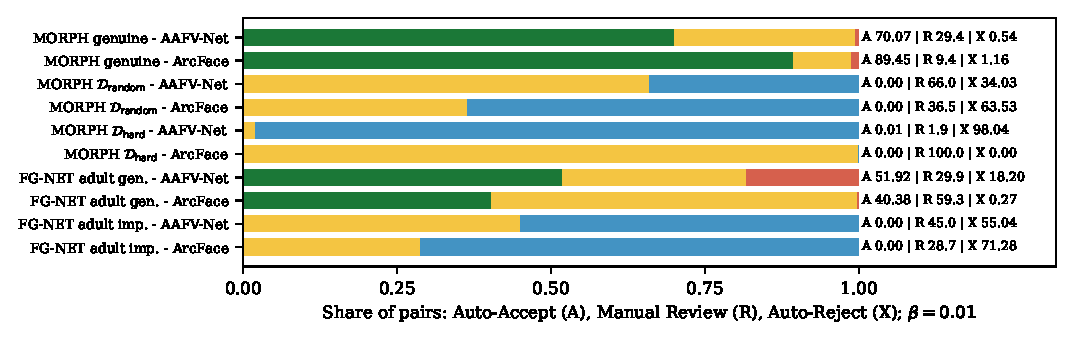
\includegraphics[width=0.85\textwidth]{figures/figR2_outcomes.pdf}
\caption{Three-way outcome shares for \sys\ and guarded ArcFace on MORPH test (Look~2) and FG-NET adults, $\beta=0.01$ set on MORPH calibration. Genuine rows: accept (green), review (yellow), false reject (orange). Impostor rows: false accept (red, near zero), review, auto-reject (blue).}
\label{fig:outcomes}
\end{figure*}

\subsection{Operational Workload}
\label{sec:workload}
Because genuine transactions dominate real streams, the review rate is driven mainly by genuine pairs. Table~\ref{tab:workload} converts the Look-2 rates into outcomes per 10,000 transactions. With 1\% impostors, \sys\ sends about 2,970 transactions to review against about 970 for guarded ArcFace, roughly three times the human workload. This holds whether impostors are random or all ArcFace-mined. \sys\ produces fewer genuine false rejects (54 versus 115). Its hard-impostor advantage converts look-alikes from review into automatic rejection, which matters only where look-alike attempts are frequent. Removing the shared-target comparisons (No Shared Targets) halves the review load (1,615) while keeping zero random and zero hard false accepts at test. On MORPH, therefore, the full system is not the best operating point among the evaluated variants. We keep it as the primary system only because it was designated in advance.

\begin{table}[t]
\centering
\caption{Operational Consequences of the Look-2 MORPH Rates ($\beta=0.01$): Expected Outcomes per 10,000 Transactions When 1\% of Transactions Are Impostors, for Three Shares of ArcFace-Mined Look-Alikes Among Impostors. Random Impostors Use $\mathcal{D}_{\text{all\_random}}$ Rates.}
\label{tab:workload}
\footnotesize
\setlength{\tabcolsep}{3pt}
\resizebox{\columnwidth}{!}{%
\begin{tabular}{@{}lccccc@{}}
\toprule
& \multicolumn{3}{c}{\textbf{Manual reviews}} & \textbf{Genuine} & \textbf{Genuine} \\
\cmidrule(lr){2-4}
\textbf{Method} & \textbf{0\% look-alike} & \textbf{10\%} & \textbf{100\%} & \textbf{auto-accepts} & \textbf{false rejects} \\
\midrule
\sys\ (Full) & 2,974 & 2,967 & 2,912 & 6,937 & 54 \\
\sys\ (No Shared Targets) & 1,615 & 1,609 & 1,551 & 8,307 & 44 \\
ArcFace Only (Guarded) & 968 & 974 & 1,030 & 8,855 & 115 \\
\bottomrule
\multicolumn{6}{@{}p{1.05\columnwidth}@{}}{\footnotesize Arithmetic on aggregate rates in \texttt{extended\_test.csv} (\texttt{a1\_look1\_posthoc.py}, part 7). No false accept was observed for any method on random impostors; the residual hard false accepts ($5/35{,}735$ for \sys) are below one per 10,000 transactions.}
\end{tabular}}
\end{table}


\subsection{Age-Gap Analysis}
\begin{table}[t]
\centering
\caption{MORPH Test (Look~2) Genuine Auto-Accept (\%) by Age-Gap Bin (\texttt{gap.py} Edges $[0,5,10,15,20,30]$ Years). Counts Are Genuine Test Pairs; 97.2\% of Them Fall in G1.}
\label{tab:gap_analysis}
\footnotesize
\setlength{\tabcolsep}{3.0pt}
\begin{tabular}{@{}lcccccc@{}}
\toprule
& \textbf{G1} & \textbf{G2} & \textbf{G3} & \textbf{G4} & \textbf{G5} & \textbf{G6} \\
\textbf{Method} & 0--4y & 5--9y & 10--14y & 15--19y & 20--29y & 30+y \\
& \scriptsize(23,631) & \scriptsize(266) & \scriptsize(184) & \scriptsize(75) & \scriptsize(137) & \scriptsize(12) \\
\midrule
\sys\ (Full) & 71.03 & 56.39 & 45.65 & 1.33 & 2.19 & 50.00 \\
ArcFace Only & 90.49 & 80.08 & 69.02 & 2.67 & 2.19 & 100.00 \\
\midrule
Difference (pp) & $-19.46$ & $-23.69$ & $-23.37$ & $-1.34$ & $0.00$ & $-50.00$ \\
\bottomrule
\multicolumn{7}{@{}p{\columnwidth}@{}}{\footnotesize G4--G6 contain 224 pairs in total; their rates are unstable. No confidence intervals per bin were saved for Look~2.}
\end{tabular}
\end{table}

Table~\ref{tab:gap_analysis} shows that ArcFace accepts more genuine pairs than \sys\ in G1--G3 (by 19.5--23.7 percentage points) and that both collapse in G4--G5. Most of the deficit arises in the guards rather than in the fused score. On the Look-1 test outputs, 97.38\% of genuine pairs exceed $T_{\text{acc}}$ before the guards are applied and 79.74\% after (Fig.~\ref{fig:diagnostics}c). ArcFace's own guards cost about 4~pp (93.58\% without versus 89.45\% with). The guards that make a zero-false-accept threshold attainable (Section~\ref{sec:ablation}) therefore also remove many genuine pairs, a direct cost of the design that a better-targeted guard might reduce. G4--G6 together contain 224 test pairs, and the training split contains few long-gap genuine pairs, so long-gap behaviour on MORPH is essentially unmeasured. Without risk--coverage curves for both methods at matched FAR, which require per-pair ArcFace scores that were not logged, we cannot claim improved cross-age verification on MORPH. The evidence points the other way.

\subsection{Hard-Impostor Analysis}
\label{sec:hard}
Look-1 outputs show that the fused score separates ArcFace-mined impostors from genuine pairs better than it separates random ones. The median $P$ is 0.0013 on $\mathcal{D}_{\text{hard}}$ against 0.0096 on $\mathcal{D}_{\text{random}}$, and 97.7\% versus 33.4\% of the two pools fall below $T_{\text{rej}}(0.01)$ (Fig.~\ref{fig:diagnostics}a). A likely cause is that half of the training negatives were mined in the same way, so $\mathcal{D}_{\text{hard}}$ is in-distribution for the fusion model; this has not been tested by ablation. The 98.04\% hard rejection should therefore not be read as general look-alike robustness; the neutral set (57.49\%) is the more representative figure. The three Look-1 hard false accepts are male pairs in G1, G2, and G1 with $P=0.980$, $0.977$, and $0.975$. Per-pair outputs were not saved for Look~2, so the five Look-2 false accepts have not been characterized, and no image of any test false accept has been inspected.

\begin{figure*}[t]
\centering
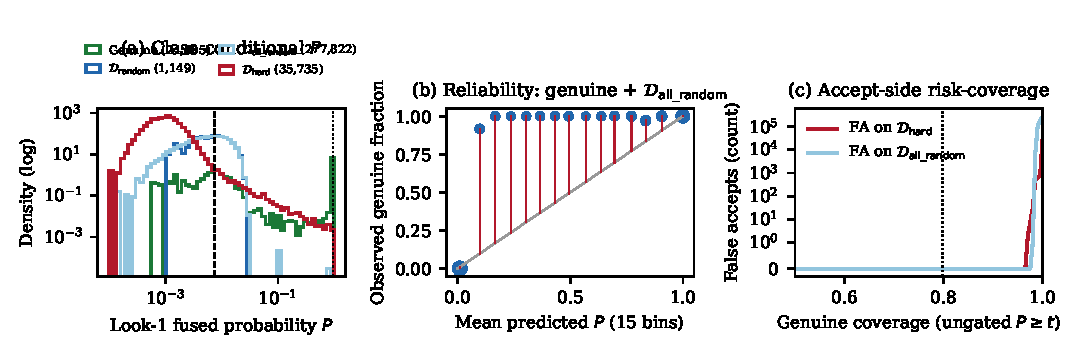
\includegraphics[width=\textwidth]{figures/figR1_posthoc_diagnostics.pdf}
\caption{Post hoc diagnostics of the Look-1 checkpoint on MORPH test (logged outputs; no parameter changed). (a) Class-conditional distributions of $P$; dashed: Look-2 $T_{\text{rej}}(0.01)$; dotted: $T_{\text{acc}}$. ArcFace-mined impostors receive lower $P$ than random impostors. (b) Reliability diagram for genuine pairs plus $\mathcal{D}_{\text{all\_random}}$; intermediate scores are strongly under-confident. (c) Genuine coverage versus false accepts when thresholding $P$ without guards; dotted line: guarded coverage 79.74\%. These curves are descriptive and were not used to set any threshold.}
\label{fig:diagnostics}
\end{figure*}

\subsection{Calibration}
\label{sec:calibration}
Table~\ref{tab:calibration} and Fig.~\ref{fig:diagnostics}b report post hoc calibration of the Look-1 $P$. The ECE is small (0.006--0.018) because almost all pairs receive $P$ near 0 or 1. The maximum bin error reaches 0.83--0.90, the calibration slope departs from 1 (0.79--1.66), and the female subgroup has an intercept of 5.02 and a slope of 2.59. Pairs with intermediate scores are almost all genuine, so $P$ is under-confident in the region that determines review. As argued in Section~\ref{sec:calib_role}, this does not affect the order-statistic guarantees, but it means $P$ should not be presented to examiners as a match probability. Calibration under dataset shift (FG-NET) and comparisons with isotonic and temperature scaling~\cite{guo2017calibration} remain to be done, because per-pair outputs were not saved for those evaluations.

\begin{table}[t]
\centering
\caption{Post Hoc Calibration Diagnostics of the Look-1 Fused Probability $P$ on MORPH Test Pairs (15 Equal-Width Bins). Absolute Calibration Depends on the Genuine Prevalence of Each Pool, So Pools Are Reported Separately. Ideal Intercept/Slope: 0/1.}
\label{tab:calibration}
\footnotesize
\setlength{\tabcolsep}{2.4pt}
\resizebox{\columnwidth}{!}{%
\begin{tabular}{@{}lrcccccc@{}}
\toprule
\textbf{Pool} & \textbf{$N$} & \textbf{Prev.} & \textbf{ECE} & \textbf{MCE} & \textbf{Brier} & \textbf{NLL} & \textbf{Int. / Slope} \\
\midrule
Genuine + $\mathcal{D}_{\text{random}}$ & 25,454 & 0.955 & 0.0180 & 0.902 & 0.0168 & 0.0786 & 2.67 / 0.79 \\
Genuine + $\mathcal{D}_{\text{all\_random}}$ & 302,127 & 0.080 & 0.0081 & 0.833 & 0.0015 & 0.0158 & 1.06 / 1.66 \\
Genuine + $\mathcal{D}_{\text{hard}}$ & 60,040 & 0.405 & 0.0060 & 0.231 & 0.0078 & 0.0365 & 1.09 / 0.92 \\
\quad Male, genuine + $\mathcal{D}_{\text{all\_random}}$ & 261,095 & 0.080 & 0.0081 & 0.883 & 0.0016 & 0.0161 & 0.41 / 1.51 \\
\quad Female, genuine + $\mathcal{D}_{\text{all\_random}}$ & 41,032 & 0.086 & 0.0078 & 0.825 & 0.0014 & 0.0136 & 5.02 / 2.59 \\
\bottomrule
\multicolumn{8}{@{}p{1.08\columnwidth}@{}}{\footnotesize Computed by \texttt{a1\_look1\_posthoc.py} from \texttt{test\_pair\_zones\_look1.csv}; no parameter was changed. Pair-level metrics; person clustering is not available in this log. Equivalent per-pair outputs were not saved for Look~2 or FG-NET, so cross-dataset calibration remains unmeasured.}
\end{tabular}}
\end{table}


\subsection{External Evaluation on FG-NET}
\label{sec:fgnet}
\begin{table*}[t]
\centering
\caption{External Evaluation on FG-NET With MORPH-Frozen Checkpoint and Thresholds ($\beta=0.01$, No Re-Tuning). Genuine Outcomes Are Auto-Accept / Review / Auto-Reject (False Reject). Adults: $a_1,a_2\ge16$ (Cut-Off Chosen Post Hoc), 1,456 Genuine and 3,670 Impostor Pairs; All Ages: 5,797 Genuine and 20,000 Impostor Pairs. Genuine Bin Counts G1--G6: Adults (405, 356, 261, 170, 186, 78); All Ages (1,654, 1,589, 1,081, 615, 572, 286). Intervals: 95\% Person-Clustered Bootstrap.}
\label{tab:fgnet}
\footnotesize
\setlength{\tabcolsep}{3.0pt}
\resizebox{\textwidth}{!}{%
\begin{tabular}{@{}llcccccccccc@{}}
\toprule
& & \multicolumn{2}{c}{\textbf{Genuine}} & \multicolumn{2}{c}{\textbf{Impostor}} & \multicolumn{6}{c}{\textbf{Genuine auto-accept by age gap (\%)}} \\
\cmidrule(lr){3-4}\cmidrule(lr){5-6}\cmidrule(l){7-12}
\textbf{Cohort} & \textbf{Method} & \textbf{Accept (\% [95\% CI])} & \textbf{Review / False rej. (\%)} & \textbf{FA} & \textbf{Auto-rej. (\%)} & $<$5y & 5--9y & 10--14y & 15--19y & 20--29y & 30+y \\
\midrule
\multirow{2}{*}{Adults} & \sys & 51.92 [44.47, 58.41] & 29.88 / \textbf{18.20} & 0 / 3,670 & 55.04 & 71.60 & 59.55 & 49.04 & 38.24 & 28.49 & 10.26 \\
 & ArcFace Only & 40.38 [34.53, 47.38] & 59.34 / 0.27 & 0 / 3,670 & 71.28 & 60.74 & 49.16 & 35.63 & 25.88 & 14.52 & 3.85 \\
\midrule
\multirow{2}{*}{All ages} & \sys & 29.86 [26.69, 33.34] & 23.44 / \textbf{46.70} & 4 / 20,000$^{\ddagger}$ & 66.44 & 59.07 & 28.95 & 14.80 & 11.71 & 9.44 & 2.80 \\
 & ArcFace Only & 21.29 [18.40, 24.22] & 76.16 / 2.55 & 0 / 20,000 & 64.42 & 45.53 & 19.19 & 9.34 & 7.32 & 4.72 & 1.05 \\
\bottomrule
\multicolumn{12}{@{}l@{}}{\footnotesize $^{\ddagger}$All four false accepts involve children aged 0--4. Bold: the MORPH-calibrated false-reject budget ($\beta=1\%$) does not transfer to FG-NET for \sys. FG-NET impostor pairs reuse images of $\le 82$ persons.}
\end{tabular}}
\end{table*}

With the MORPH checkpoint and thresholds unchanged (Table~\ref{tab:fgnet}), \sys\ accepts 51.92\% of adult genuine pairs against 40.38\% for ArcFace, is higher in every age-gap bin, and produces no false accept among 3,670 adult impostor pairs. Two negative results qualify this. First, the reject threshold does not transfer: \sys\ falsely auto-rejects 18.20\% of adult genuine pairs (46.70\% at all ages) against a design target of 1\%, while ArcFace rejects 0.27\%. The FG-NET gain in automation is therefore partly obtained by deciding wrongly rather than deferring. Second, at all ages \sys\ produces four false accepts in 20,000 impostor pairs, all involving children aged 0--4, which motivated the post hoc adult restriction. FG-NET contains 82 persons, so the adult interval [44.47, 58.41] is wide, and the impostor counts are not independent trials. Shift-aware threshold selection, for example weighted conformal calibration~\cite{tibshirani2019covshift}, is a direct remedy that we have not implemented.

\subsection{Ablations}
\label{sec:ablation}
\begin{table}[t]
\centering
\caption{Component and Guard Ablation Study on Calibration Common Subset ($\beta = 1.0\%$, $N_{\text{same}} = 1{,}500$, $N_{\text{hard}} = 1{,}500$; \texttt{decision\_table\_calibration.csv}).}
\label{tab:ablations}
\footnotesize
\setlength{\tabcolsep}{3.5pt}
\resizebox{\columnwidth}{!}{%
\begin{tabular}{@{}lcccc@{}}
\toprule
\textbf{Ablation Variant} & \textbf{$T_{\text{acc}}$} & \textbf{Acc. (\%)} & \textbf{Rej. (\%)} & \textbf{Rand. Rej. (\%)} \\
\midrule
\textbf{Full \sys\ ($\rho=0.20$)} & 0.956 & 74.13 & \textbf{98.20} & 26.15 \\
\midrule
\textit{Metric Ablations:} & & & & \\
Drop ArcFace & 0.994 & 0.73 & 17.87 & 52.99 \\
ArcFace Score Only & 1.008 & 0.00 & 97.73 & 24.19 \\
Drop LPIPS & 1.000 & 62.87 & 97.47 & 29.32 \\
Drop SSIM & 0.989 & 72.80 & 97.40 & 23.68 \\
Drop VGG-Face & 0.976 & 73.93 & 97.20 & 19.57 \\
Drop EfficientNet & 0.978 & 81.27 & 97.60 & 20.85 \\
\midrule
\textit{Architecture \& Guard Ablations:} & & & & \\
No Branch Masking ($p=0$)$^\ast$ & 0.593 & 3.60 & 98.40 & 30.94 \\
No Context ($g,Q,R_{\text{sam}}$) & 1.042 & 0.00 & 98.07 & 24.70 \\
No Reliability ($R_{\text{sam}}$) & 0.989 & 73.27 & 97.80 & 23.85 \\
No Pair Weights & 0.985 & 74.40 & 97.33 & 24.62 \\
Forward Target Only & 0.954 & 75.07 & 98.27 & 25.98 \\
No Shared Targets & 0.997 & \textbf{84.80} & 98.27 & 29.23 \\
Shared Targets Only & 1.024 & 0.00 & 98.13 & 19.06 \\
Direct-Only MLP & 1.042 & 0.00 & 98.47 & 26.67 \\
SAM-Only MLP & 1.001 & 0.00 & 44.80 & \textbf{60.77} \\
Fusion LogReg (No MLP) & 0.869 & 64.67 & 0.00 & 57.86 \\
No Probability Guards (All 3)$^\ddagger$ & 1.005 & 0.00 & 98.20 & 26.15 \\
\bottomrule
\multicolumn{5}{@{}l@{}}{\footnotesize $^\ast$Selected $\rho = 0.35$ in calibration grid; $^\ddagger$\texttt{guard\_none}, \texttt{guard\_quality\_only},}\\
\multicolumn{5}{@{}l@{}}{\footnotesize and \texttt{guard\_quality\_reliability} produced identical rates.}
\end{tabular}%
}
\end{table}

Table~\ref{tab:ablations} (calibration subset, development data) shows four effects.
\begin{itemize}
\item \emph{Guards.} Removing the probability floors gives $T_{\text{acc}}=1.005$ and 0\% acceptance in all three guard ablations.
\item \emph{Masking and context.} Without SAM masking, acceptance falls to 3.60\%; without $g$, $Q$, and $R_{\text{sam}}$ it is 0\%.
\item \emph{Similarity measures.} ArcFace is indispensable (0.73\% without it), LPIPS contributes 11.3~pp, and dropping EfficientNet \emph{raises} acceptance to 81.27\%. EfficientNet is therefore redundant; it is retained only because the frozen checkpoints use it.
\item \emph{Removing $R_{\text{sam}}$} changes acceptance by less than 1~pp. Its contribution is through the guard, not the fusion input.
\end{itemize}
Removing shared targets raises acceptance to 84.80\%; on test, its neutral rejection (53.98\% [51.77, 56.18]) overlaps that of the full system (57.49\% [55.34, 59.73]).

\begin{table*}[t]
\centering
\caption{Calibration Split Discrimination and Three-Way Decision Comparison ($\beta = 1.0\%$). Ranking metrics are computed on full calibration $\mathcal{D}_{\text{hard}}$ ($N=35{,}769$) except VLM ($N=1{,}500$). Decision rates come from the label-free calibration common subset ($N_{\text{same}}=1{,}500$, $N_{\text{random}}=1{,}170$, $N_{\text{hard}}=1{,}500$; \texttt{decision\_table\_calibration.csv}).}
\label{tab:cal_subset}
\footnotesize
\setlength{\tabcolsep}{4.5pt}
\begin{tabular}{@{}lccccccc@{}}
\toprule
\textbf{Architecture} & \makecell{\textbf{Cal. AUC}\\\textbf{($\mathcal{D}_{\text{hard}}$)}} & \makecell{\textbf{TPR @}\\\textbf{$\text{FPR}=10^{-3}$}} & \makecell{\textbf{Frozen}\\\textbf{$T_{\text{acc}}$}} & \makecell{\textbf{Same Accept}\\\textbf{(\%)}} & \makecell{\textbf{Random Rej.}\\\textbf{(\%)}} & \makecell{\textbf{Hard Rej.}\\\textbf{(\%)}} & \makecell{\textbf{Eval. Pool}\\\textbf{($N_{\text{hard}}$ AUC)}} \\
\midrule
\textbf{\sys\ (Full)} & \textbf{0.998} & \textbf{0.973} & 0.956 & 74.13 & 26.15 & \textbf{98.20} & Full Cal. (35,769) \\
ArcFace Only (Guarded) & 0.980 & 0.969 & 0.850 & \textbf{87.20} & 47.95 & 0.00 & Full Cal. (35,769) \\
Direct 5-Score LogReg & 0.981 & 0.971 & 0.913 & 84.27 & \textbf{57.26} & 0.00 & Full Cal. (35,769) \\
Direct-Only MLP & 0.998 & 0.971 & 1.042 & 0.00 & 26.67 & 98.47 & Full Cal. (35,769) \\
Siamese CNN (ResNet-18) & 0.953 & 0.311 & 0.982 & 0.27 & 49.74 & 10.87 & Full Cal. (35,769) \\
Siamese ViT (ViT-B/16) & 0.972 & 0.605 & 1.001 & 0.00 & 51.97 & 12.20 & Full Cal. (35,769) \\
VLM (Qwen2-VL-2B LoRA) & 0.906 & 0.054 & 0.998 & 0.00 & 47.01 & 10.20 & Common Subset (1,500) \\
\bottomrule
\end{tabular}
\end{table*}



\subsection{Demographic Analysis}
\begin{table}[t]
\centering
\caption{Sex-Disaggregated Verification Audit on Protected MORPH Test Split (Look 1 Log \texttt{test\_pair\_zones\_look1.csv}; Per-Pair Sex Metadata Was Not Saved in Look 2).}
\label{tab:fairness}
\footnotesize
\setlength{\tabcolsep}{3.5pt}
\resizebox{\columnwidth}{!}{%
\begin{tabular}{@{}lcccc@{}}
\toprule
\textbf{Cohort} & \makecell{\textbf{Same Accept}\\\textbf{(\%)}} & \makecell{\textbf{Same Review}\\\textbf{(\%)}} & \makecell{\textbf{Random FA}\\\textbf{$\mathcal{D}_{\text{random}}$}} & \makecell{\textbf{Hard FA}\\\textbf{$\mathcal{D}_{\text{hard}}$}} \\
\midrule
Male ($N_{\text{same}}=20{,}774$) & 81.07 & 18.93 & 0 / 982 & 3 / 30,921 \\
Female ($N_{\text{same}}=3{,}531$) & 71.93 & 28.07 & 0 / 167 & 0 / 4,814 \\
\midrule
Gap ($\Delta$ M$-$F / DI Ratio) & \multicolumn{2}{c}{9.14 pp (Ratio: 0.887)} & 0.00 pp & -- \\
\bottomrule
\end{tabular}%
}
\end{table}

Per-pair sex was logged only at Look~1 (Table~\ref{tab:fairness}). Male genuine pairs were auto-accepted at 81.07\% (20,774 pairs) and female pairs at 71.93\% (3,531), a gap of 9.14~pp. Within G1 the rates are 82.34\% [81.81, 82.86] and 72.05\% [70.54, 73.52] (pair-level Wilson intervals, which understate person-level uncertainty). No random-impostor false accept occurred in either group (0/982, 0/167). All three Look-1 hard false accepts were male. Race, age group, and intersectional subgroups were not analysed, although MORPH provides race labels; this analysis is required (Section~\ref{sec:limitations}).

\subsection{Computational Cost}
\begin{table}[t]
\centering
\caption{Trainable Parameters and Per-Pair Work. Wall-Clock Timings Were Not Logged in the Repository and Are Therefore Not Reported (Required Experiment E10).}
\label{tab:complexity}
\footnotesize
\setlength{\tabcolsep}{3.5pt}
\resizebox{\columnwidth}{!}{%
\begin{tabular}{@{}lcc@{}}
\toprule
\textbf{Stage} & \textbf{Trainable params} & \textbf{Work per pair} \\
\midrule
Detection, alignment, quality & 0 (pre-trained / analytic) & 2 images \\
Direct similarity (5 measures) & 0 (frozen) & 1 comparison, 4 networks \\
SAM synthesis + reliability & 0 (frozen) & up to $2+2K\le16$ generated faces \\
Linear heads $W_d,W_s,W_f$ & $3\times6=18$ (12 effective) & 3 dot products \\
Fusion MLP $11\!\to\!32\!\to\!16\!\to\!1$ & 929 & 1 forward pass \\
5-seed ensemble + Platt scalers & $5\times947+6=4{,}741$ & 5 forward passes \\
\bottomrule
\end{tabular}}
\end{table}

Table~\ref{tab:complexity} lists what was measured. The fusion stage is negligible in size (947 parameters per seed). The dominant cost is SAM synthesis, which renders up to $2+2K\le16$ faces per pair. End-to-end latency, its 95th percentile, throughput, memory, and the cost of a cascade that invokes SAM only for non-decided pairs were not measured. Earlier drafts quoted per-stage latencies; we do not repeat them here, because the logs that produced them could not be located.

% =====================================================================================
\section{Discussion}
\label{sec:discussion}
\textbf{What the evidence supports.} For MORPH-like adult random impostors, the accept rule carries a finite-sample certificate obtained from calibration data alone, and a held-out audit agrees. Branch-probability guards are what make a zero-false-accept threshold usable for a fused score whose impostor tail otherwise reaches 1. A reliability-gated synthetic branch can be included without destabilizing the accept threshold, provided it is masked during training.

\textbf{What it does not support.} The current evidence does not show that age-progression evidence improves cross-age verification. On MORPH the full system accepts fewer genuine pairs than ArcFace in every populated age-gap bin and creates about three times the review workload. The strong hard-impostor rejection is plausibly a consequence of training on similarly mined negatives. The FG-NET gains come with a large, uncontrolled false-reject rate. These observations shift the paper's contribution from a better verifier to a risk-controlled decision protocol, and they identify the experiments that would decide whether the synthetic branch has value: matched-FAR risk--coverage comparisons with per-pair scores, an ablation without hard training negatives, and evaluation on large-gap external benchmarks.

\textbf{Relation to AIFR.} AIM and OrdCon improve the representation and evaluate on large-gap protocols (youngest versus oldest image per subject) and several datasets~\cite{zhao2022aim,wang2025ordcon}. Our MORPH protocol is dominated by short gaps, and our external evidence rests on 82 FG-NET persons. A fair comparison would place an AIFR embedding inside the same decision protocol and report coverage, review, and certified FAR on AgeDB~\cite{moschoglou2017agedb}, CACD-VS~\cite{chen2014cacd}, and CALFW~\cite{zheng2017calfw}.

% =====================================================================================
\section{Limitations and Required Work}
\label{sec:limitations}
\begin{enumerate}
\item \emph{Test adaptivity.} Whether Look-1 results influenced the changes before Look~2 cannot be established. A confirmatory evaluation on an untouched external set, with a pre-registered analysis plan, is required.
\item \emph{FAR scale.} The certificate and audit support FAR on the order of $3\times10^{-3}$, not $10^{-4}$ (Table~\ref{tab:samplesize}). They do not cover look-alikes, other capture conditions, or children.
\item \emph{External validity.} Only FG-NET (82 persons) was used, with a post hoc adult cut-off. The reject threshold failed to transfer.
\item \emph{Identity preservation.} SAM outputs were not evaluated with a recognizer outside the pipeline or by human raters. $R_i$ uses ArcFace, which is also a fusion input. Only one generator was used.
\item \emph{Baselines.} AdaFace, MagFace, AIFR models, a converged Siamese ViT, and generic selective classifiers are missing. Risk--coverage curves at matched FAR are missing because per-pair baseline scores were not logged.
\item \emph{Hard impostors.} The five Look-2 false accepts are uncharacterized. The effect of mined training negatives is untested.
\item \emph{Fairness.} The analysis covers sex only, at Look~1, with pair-level intervals; race, age-group, and intersectional analyses and subgroup calibration are missing.
\item \emph{Robustness and cost.} There are no degradation, missing-branch, or attack experiments, and no end-to-end latency, memory, or cascade measurements.
\item \emph{Data hygiene assumptions.} The quarantine relies on an identifier-suffix rule (with an ArcFace-centroid check), and the calibration procedure allowed label corrections after inspecting the highest-scoring calibration impostors. If any removed or relabelled pair was a true impostor, both the certificate and the audit would be optimistic. A record of all corrections should accompany the paper.
\item \emph{Design debt.} Four constant input slots and a redundant similarity measure (EfficientNet) remain because the frozen checkpoints use them.
\end{enumerate}

% =====================================================================================
\section{Conclusion}
\label{sec:conclusion}
We framed adult cross-age face verification as a three-way decision and showed that \sys's accept rule yields a distribution-free random-impostor FAR certificate from calibration data ($0.349\%$ at 95\% confidence), consistent with a held-out audit (0/1,149). Branch-probability guards are essential for making such a rule usable on a fused score. The evaluation also shows that, on MORPH, the system accepts fewer genuine pairs and requires more manual review than a guarded ArcFace baseline, that its strongest look-alike result may reflect its training negatives, and that its false-reject control does not survive transfer to FG-NET. The next steps are a confirmatory external evaluation, shift-aware threshold calibration, independent validation of the generated evidence, and matched-FAR comparisons with modern and age-invariant recognizers.

\section*{Acknowledgments and Disclosures}
[Funding statement and CRediT roles to be confirmed by the authors.] The authors declare no conflicts of interest. Experiments use existing academic datasets (MORPH Album~2 and FG-NET) under their licence terms; no new data were collected. \texttt{InsightFace}, SAM, and the age estimator carry non-commercial licences.

\appendices
\section{Person-Clustered Bootstrap Intervals (MORPH Test, Look~2)}
\begin{table}[t]
\centering
\caption{Complete 95\% Subject-Clustered Bootstrap Confidence Intervals (500 Resamples) on MORPH \texttt{test} Split ($\beta = 1.0\%$, \texttt{extended\_test.csv}).}
\label{tab:supp_intervals}
\footnotesize
\setlength{\tabcolsep}{2.8pt}
\begin{tabular}{@{}lccc@{}}
\toprule
\textbf{Method} & \makecell{\textbf{Same Accept}\\\textbf{95\% CI (\%)}} & \makecell{\textbf{Hard Reject}\\\textbf{95\% CI (\%)}} & \makecell{\textbf{Neutral Reject}\\\textbf{95\% CI (\%)}} \\
\midrule
\textbf{\sys\ (Full)} & [66.52, 73.11] & [97.77, 98.31] & [55.34, 59.73] \\
No Shared Targets & [82.03, 85.72] & [97.57, 98.12] & [51.77, 56.18] \\
ArcFace Only (Guarded) & [88.03, 90.65] & [0.00, 0.00] & [26.58, 30.40] \\
ArcFace (No Guards) & [92.41, 94.86] & [0.00, 0.00] & [26.61, 30.54] \\
Direct 5-Score LogReg & [85.39, 88.65] & [0.00, 0.00] & [20.64, 24.21] \\
Direct-Only MLP & [0.00, 0.00] & [97.46, 98.07] & [47.73, 52.20] \\
Siamese CNN (ResNet-18) & [0.13, 0.30] & [9.37, 10.43] & n/a \\
Siamese ViT (ViT-B/16) & [0.00, 0.00] & [9.43, 10.69] & n/a \\
\bottomrule
\end{tabular}
\end{table}


Table~\ref{tab:supp_intervals} gives the 95\% person-clustered bootstrap intervals (500 resamples) for the methods of Table~\ref{tab:main_results}.

\bibliographystyle{IEEEtran}
\bibliography{references}

\end{document}
